\def\bmode{2} % Mode 0 for presentation, mode 1 for a handout with notes, mode 2 for handout without notes
\if 0\bmode
\documentclass[smaller]{beamer}
\else \if 1\bmode
\immediate\write18{pdflatex -jobname=\jobname-Notes-Handout\space\jobname}
\documentclass[smaller,handout]{beamer}
\usepackage{handoutWithNotes}
\pgfpagesuselayout{2 on 1 with notes}[letterpaper, landscape, border shrink=4mm]
\else \if 2\bmode
\immediate\write18{pdflatex -jobname=\jobname-Handout\space\jobname}
\documentclass[smaller,handout]{beamer}
\fi
\fi
\fi
%\documentclass[smaller]{beamer}

% \documentclass[smaller,handout
% ]{beamer}
%\usepackage{etex}
%\newcommand{\num}{6{} }

% \usetheme[
%   outer/progressbar=foot,
%   outer/numbering=counter,
%  block=fillFF
% ]{metropolis}

%\useoutertheme{metropolis}

\usetheme{Madrid}
\useoutertheme[subsection=false]{miniframes} % Alternatively: miniframes, infolines, split
\useinnertheme{circles}
\usecolortheme{seahorse}

\usepackage[backend=biber,style=authoryear,maxcitenames=2,maxbibnames=99,safeinputenc,url=false,
eprint=false]{biblatex}
\addbibresource{bib/references.bib}
\AtEveryCitekey{\iffootnote{{\tiny}\tiny}{\tiny}}
\usepackage{appendixnumberbeamer}
%\usepackage{pgfpages}
%\setbeameroption{hide notes} % Only slides
%\setbeameroption{show only notes} % Only notes
%\setbeameroption{hide notes} % Only notes
%\setbeameroption{show notes on second screen=right} % Both

% \usepackage[sfdefault]{Fira Sans}

% \setsansfont[BoldFont={Fira Sans}]{Fira Sans Light}
% \setmonofont{Fira Mono}

%\usepackage{fira}
%\setsansfont{Fira}
%\setmonofont{Fira Mono}
% To give a presentation with the Skim reader (http://skim-app.sourceforge.net) on OSX so
% that you see the notes on your laptop and the slides on the projector, do the following:
% 
% 1. Generate just the presentation (hide notes) and save to slides.pdf
% 2. Generate onlt the notes (show only nodes) and save to notes.pdf
% 3. With Skim open both slides.pdf and notes.pdf
% 4. Click on slides.pdf to bring it to front.
% 5. In Skim, under "View -> Presentation Option -> Synhcronized Noted Document"
%    select notes.pdf.
% 6. Now as you move around in slides.pdf the notes.pdf file will follow you.
% 7. Arrange windows so that notes.pdf is in full screen mode on your laptop
%    and slides.pdf is in presentation mode on the projector.

% Give a slight yellow tint to the notes page
%\setbeamertemplate{note page}{\pagecolor{yellow!5}\insertnote}\usepackage{palatino}


%\usetheme{metropolis}
%\usecolortheme{beaver}
\usepackage{xcolor}
\definecolor{darkcandyapplered}{HTML}{A40000}
\definecolor{lightcandyapplered}{HTML}{e74c3c}

%\setbeamercolor{title}{fg=darkcandyapplered}
%\setbeamercolor{frametitle}{bg=darkcandyapplered!80!black!90!white}
%\setbeamertemplate{frametitle}{\bf\insertframetitle}
%\setbeamercolor{footnote mark}{fg=darkcandyapplered}
%\setbeamercolor{footnote}{fg=darkcandyapplered!70}
%\Raggedbottom
%\setbeamerfont{page number in head/foot}{size=\tiny}
%\usepackage[tracking]{microtype}


\setbeamertemplate{frametitle}{%
    \nointerlineskip%
    \begin{beamercolorbox}[wd=\paperwidth,ht=2.0ex,dp=0.6ex]{frametitle}
        \hspace*{1ex}\insertframetitle%
    \end{beamercolorbox}%
}



\setbeamerfont{caption}{size=\footnotesize}
\setbeamercolor{caption name}{fg=darkcandyapplered}


%\usepackage[sc,osf]{mathpazo}   % With old-style figures and real smallcaps.
%\linespread{1.025}              % Palatino leads a little more leading

% Euler for math and numbers
%\usepackage[euler-digits,small]{eulervm}
%\AtBeginDocument{\renewcommand{\hbar}{\hslash}}
\usepackage{graphicx,multirow,paralist,booktabs}


%\mode<presentation> { \setbeamercovered{transparent} }

\setbeamertemplate{navigation symbols}{}
\makeatletter
\def\beamerorig@set@color{%
  \pdfliteral{\current@color}%
  \aftergroup\reset@color
}
\def\beamerorig@reset@color{\pdfliteral{\current@color}}
\makeatother

%=== GRAPHICS PATH ===========
\graphicspath{{./m4-images/}}
% Marginpar width
%Marginpar width
%\setlength{\marginparsep}{.02in}


%% Captions
% \usepackage{caption}
% \captionsetup{
%   labelsep=quad,
%   justification=raggedright,
%   labelfont=sc
% }

%AMS-TeX packages

\usepackage{amssymb,amsmath,amsthm} 
\usepackage{bm}
\usepackage{color}

\usepackage{hyperref,enumerate}
\usepackage{minitoc,array}


%https://tex.stackexchange.com/a/31370/2269
\usepackage{mathtools,cancel}

\renewcommand{\CancelColor}{\color{red}} %change cancel color to red

\makeatletter
\let\my@cancelto\cancelto %copy over the original cancelto command
\newcommand<>{\cancelto}[2]{\alt#3{\my@cancelto{#1}{#2}}{\mathrlap{#2}\phantom{\my@cancelto{#1}{#2}}}}
% redefine the cancelto command, using \phantom to assure that the
% result doesn't wiggle up and down with and without the arrow
\makeatother


\definecolor{slblue}{rgb}{0,.3,.62}
\hypersetup{
    colorlinks,%
    citecolor=blue,%
    filecolor=blue,%
    linkcolor=blue,
    urlcolor=slblue
}

%%% TIKZ
\usepackage{animate}
\usepackage{tikz}
\usepackage{pgfplots}
\usepackage{pgfplotstable}
\usepackage{pgfgantt}
\usepackage{tikzsymbols}
\pgfplotsset{compat=newest}
\usepgfplotslibrary{groupplots,fillbetween}

\usetikzlibrary{arrows,shapes,positioning,shapes.geometric}
\usetikzlibrary{decorations.markings}
\usetikzlibrary{shadows,automata}
\usetikzlibrary{patterns,matrix}
\usetikzlibrary{trees,mindmap,backgrounds}
%\usetikzlibrary{circuits.ee.IEC}
\usetikzlibrary{decorations.text}
% For Sagnac Picture
\usetikzlibrary{%
    decorations.pathreplacing,%
    decorations.pathmorphing%
}
\tikzset{no shadows/.style={general shadow/.style=}}
%
%\usepackage{paralist}



%%% FORMAT PYTHON CODE
%\usepackage{listings}
% Default fixed font does not support bold face
\DeclareFixedFont{\ttb}{T1}{txtt}{bx}{n}{8} % for bold
\DeclareFixedFont{\ttm}{T1}{txtt}{m}{n}{8}  % for normal

% Custom colors
\definecolor{deepblue}{rgb}{0,0,0.5}
\definecolor{deepred}{rgb}{0.6,0,0}
\definecolor{deepgreen}{rgb}{0,0.5,0}
 

%\usepackage{listings}

% Python style for highlighting
% \newcommand\pythonstyle{\lstset{
% language=Python,
% basicstyle=\footnotesize\ttm,
% otherkeywords={self},             % Add keywords here
% keywordstyle=\footnotesize\ttb\color{deepblue},
% emph={MyClass,__init__},          % Custom highlighting
% emphstyle=\footnotesize\ttb\color{deepred},    % Custom highlighting style
% stringstyle=\color{deepgreen},
% frame=tb,                         % Any extra options here
    % showstringspaces=false            % 
% }}

% % Python environment
% \lstnewenvironment{python}[1][]
% {
% \pythonstyle
% \lstset{#1}
% }
% {}

% % Python for external files
% \newcommand\pythonexternal[2][]{{
% \pythonstyle
% \lstinputlisting[#1]{#2}}}

% Python for inline
% 
% \newcommand\pythoninline[1]{{\pythonstyle\lstinline!#1!}}


\newcommand{\osn}{\oldstylenums}
\newcommand{\dg}{^{\circ}}
\newcommand{\lt}{\left}
\newcommand{\rt}{\right}
\newcommand{\pt}{\phantom}
\newcommand{\tf}{\therefore}
\newcommand{\?}{\stackrel{?}{=}}
\newcommand{\fr}{\frac}
\newcommand{\dfr}{\dfrac}
\newcommand{\ul}{\underline}
\newcommand{\tn}{\tabularnewline}
\newcommand{\nl}{\newline}
\newcommand\relph[1]{\mathrel{\phantom{#1}}}
\newcommand{\cm}{\checkmark}
\newcommand{\ol}{\overline}
\newcommand{\rd}{\color{red}}
\newcommand{\bl}{\color{blue}}
\newcommand{\pl}{\color{purple}}
\newcommand{\og}{\color{orange!90!black}}
\newcommand{\gr}{\color{green!40!black}}
\newcommand{\nin}{\noindent}
\newcommand{\la}{\lambda}
\renewcommand{\th}{\theta}
\newcommand{\al}{\alpha}
\newcommand{\G}{\Gamma}
\newcommand*\circled[1]{\tikz[baseline=(char.base)]{
            \node[shape=circle,draw,thick,inner sep=1pt] (char) {\small #1};}}

\newcommand{\bc}{\begin{compactenum}[\quad--]}
\newcommand{\ec}{\end{compactenum}}

\newcommand{\p}{\partial}
\newcommand{\pd}[2]{\frac{\partial{#1}}{\partial{#2}}}
\newcommand{\dpd}[2]{\dfrac{\partial{#1}}{\partial{#2}}}
\newcommand{\pdd}[2]{\frac{\partial^2{#1}}{\partial{#2}^2}}
\newcommand{\nmfr}[3]{\Phi\left(\frac{{#1} - {#2}}{#3}\right)}


\pgfmathdeclarefunction{poiss}{1}{%
  \pgfmathparse{(#1^x)*exp(-#1)/(x!)}%
  }

\pgfmathdeclarefunction{gauss}{2}{%
  \pgfmathparse{1/(#2*sqrt(2*pi))*exp(-((x-#1)^2)/(2*#2^2))}%
}

\pgfmathdeclarefunction{expo}{2}{%
  \pgfmathparse{#1*exp(-#1*#2)}%
}

\pgfmathdeclarefunction{expocdf}{2}{%
  \pgfmathparse{1 -exp(-#1*#2)}%
}

% \makeatletter
% \long\def\ifnodedefined#1#2#3{%
%     \@ifundefined{pgf@sh@ns@#1}{#3}{#2}%
% }

% \pgfplotsset{
%     discontinuous/.style={
%     scatter,
%     scatter/@pre marker code/.code={
%         \ifnodedefined{marker}{
%             \pgfpointdiff{\pgfpointanchor{marker}{center}}%
%              {\pgfpoint{0}{0}}%
%              \ifdim\pgf@y>0pt
%                 \tikzset{options/.style={mark=*, fill=white}}
%                 \draw [densely dashed] (marker-|0,0) -- (0,0);
%                 \draw plot [mark=*] coordinates {(marker-|0,0)};
%              \else
%                 \tikzset{options/.style={mark=none}}
%              \fi
%         }{
%             \tikzset{options/.style={mark=none}}        
%         }
%         \coordinate (marker) at (0,0);
%         \begin{scope}[options]
%     },
%     scatter/@post marker code/.code={\end{scope}}
%     }
% }

% \makeatother

\renewcommand{\arraystretch}{1.5}
%%%%%%%%%%%%%%%%%%%%%%%%%%%%%%%%%%%%%%%%%%%%%%%%%%%
%%%%%%%%%%%%%%%%%%%%%%%%%%%%%%%%%%%%%%%%%%%%%%%%%%%

\title[CEE 260/MIE 273 M4c: Hypothesis Testing]{{\normalsize CEE 260/MIE 273: Probability and Statistics in Civil Engineering} \\
Lecture M4c: Hypothesis Testing and p-values}
\date[\today]{\footnotesize \today}
\author{{\bf Jimi Oke}}
\institute[UMass Amherst]{
  \begin{tikzpicture}[baseline=(current bounding box.center)]
    \node[anchor=base] at (-7,0) (its) {
\includegraphics[scale=.3]{UMassEngineering_vert}} ;
  \end{tikzpicture}
}


    
\begin{document}

\maketitle




\begin{frame}
  \frametitle{Outline}
  \tableofcontents
\end{frame}

\begin{frame}
  \frametitle{Today's objectives}
  \pause

  \begin{itemize}
  \item Learn how to conduct a hypothesis test on the mean of a population
    \pause
    
  \item Know when to use a lower-tailed, upper-tailed or two-tailed test
    \pause

  \item Understand Type I errors and their relationship to $p$-values
    \pause
    
  \item Learn how to use $p$-values to conduct a hypothesis test
  \end{itemize}
\end{frame}

\section{Hypothesis testing}

\begin{frame}
  \frametitle{Hypothesis testing}\pause
  \begin{itemize}
  \item Hypothesis testing provides a framework for evaluating parameter(s) of a population with respect to a desired or
    known outcome.

  \item Given that the in most cases, we can only estimate these parameters, hypothesis testing allows us to determine
    if the estimate supports a \textbf{research hypothesis}.

  \item  The results of this testing is useful for \textbf{decision-making}.
\end{itemize}

\end{frame}



\begin{frame}
  \frametitle{Formulating a hypothesis test}\pause
  A hypothesis is a statement regarding a parameter.\\

  In a test, there are usually two competing hypotheses:\pause
  \begin{itemize}
  \item $H_0$: \pause the \textbf{null} hypothesis
  \item $H_1$: \pause the \textbf{alternative} hypothesis ($H_A$ is also used to denote this)
  \end{itemize}
  \pause

  The null hypothesis is usually framed as an equality, i.e.:
  \begin{equation}
    \label{eq:10}
    H_0: p = p_0
  \end{equation}
  where $p_0$ is the specified standard.

  The alternative is given by\pause
  \begin{equation}
    \label{eq:11}
    H_1: p \ne p_0
  \end{equation}
  
\end{frame}

\begin{frame}
  \frametitle{Outcomes of a hypothesis test}\pause
  The null hypothesis is presumed  unless there is sufficient evidence to discard it.{} \pause
  The alternative hypothesis, however, is what we hope to support.\pause
  \medskip
  
  \begin{quote}
  \rd  In experimental design, we frame the null hypothesis in such a way as to reject it.
  \end{quote}

  \pause
  Thus there are \textbf{two outcomes} of a hypothesis test:

  \begin{itemize}[<+->]
  \item {\bf Reject $\bm{H_0}$}: \pause
    because of sufficient sample evidence in support of $H_1$
  \item {\bf Fail to reject $\bm{H_0}$}: \pause
    because of insufficient evidence in support of $H_1$
  \end{itemize}
  
  \pause

  \medskip
  
  \begin{alertblock}{No truth test for the null hypothesis}
    The failure to reject $H_0$ does not mean that $H_0$ is true.
  \end{alertblock}
  
\end{frame}

\begin{frame}
  \frametitle{Further explanation of hypothesis test outcomes}
  \begin{exampleblock}{Example 1: Outcome of a trial}\pause
    In a jury trial, the hypotheses are:
    \begin{itemize}
    \item $H_0$: defendant is innocent
    \item $H_1$: defendant is guilty (not innocent)
    \end{itemize}
    \pause
    
    The null hypothesis $H_0$ is \textbf{rejected} if there evidence beyond reasonable
    doubt that the defendant is guilty.  \pause

    However, \alert{\bf failure to reject} $H_0$ does not imply the defendant is
    innocent, only that there is\textbf{ insufficient evidence to prove otherwise}.
  \end{exampleblock}
\end{frame}



\begin{frame}
  \frametitle{Hypothesis testing in practice}
  \begin{exampleblock}{Example 2: Chip manufacturing}
    \pause
    A company manufacturing RAM chips claims the defective rate of the population is 5\%.
    Using a 500-chip sample from production, formulate a  hypothesis test to evaluate the validity of the company's claim.\\
    \pause
    Let $p$ denote the {\it true} defective probability.\\
    \pause
    We structure our hypothesis test as follows:\pause
    \begin{eqnarray*}
      H_0: p = 0.05 \\
      H_1: p > 0.05
    \end{eqnarray*}
    \pause
    {\rd Note: this is a one-sided hypothesis test (testing in one direction only)}
  \end{exampleblock}
\end{frame}


\begin{frame}
  \frametitle{Hypothesis testing in practice}
  \begin{exampleblock}{Example 2: Chip manufacturing (cont.)}\pause
    In order to test the hypotheses, we must choose a \textbf{test statistic}.\\\pause
    
    Here, we let $X$ denote the number of defective chips in the sample of 1000.\\
    \pause
    
    Then in order to determine whether or not to reject $H_0$, \pause
    we must decide on a \textbf{critical value}.

    We note that this is a Bernoulli process.{} \pause Thus, if $p=0.05$, then the
    expected number of defective chips is
    \begin{equation*}
      \ol{X}= np = 1000\times0.05 = 50
    \end{equation*}
    \pause      
    Say the critical value were $p^{*} = .1$, then $ p \ge .1$ could then be considered
    as strong evidence that $p > 0.05$.
    
  \end{exampleblock}
\end{frame}


\begin{frame}
  \frametitle{Hypothesis testing in practice}
  \begin{exampleblock}{Example 2: Chip manufacturing (cont.)}\pause
    
    Thus, we would reject $H_0$.

    \pause

    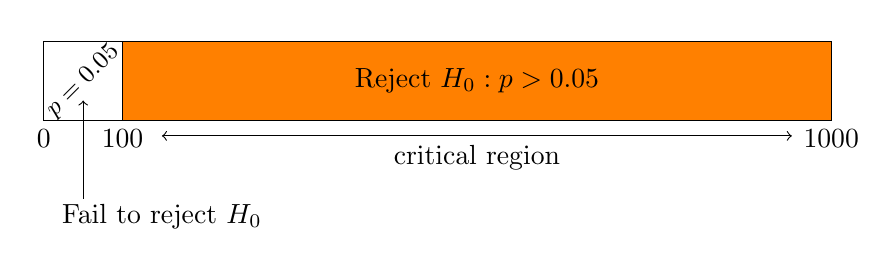
\begin{tikzpicture}[]
      \draw (0,0) rectangle (1,1) node[pos=.5,rotate=45] {\small $p = 0.05$};
      \draw[fill=orange] (1,0) rectangle (10,1) node[pos=.5] {Reject $H_0: p > 0.05$};
      \node[below] at (0,0) {0};
      \node[below] at (1,0) {100};
      \node[below] at (10,0) {1000};
      \draw[<->] (1.5,-0.2) -- node[below] {critical region} (9.5,-0.2);
      \node[above] at (1.5,-1.5) {Fail to reject $H_0$};
      \draw[->] (.5,-1) -- (.5,.25);
    \end{tikzpicture}
  \end{exampleblock}
\end{frame}


\begin{frame}
  \frametitle{Errors in hypothesis testing}\pause
  Since we are working with finite samples, errors are bound to occur in decision-making.\\

  \bigskip
  
  \pause

  The decision matrix is:\pause

  \begin{center}
  \begin{tabular}{|c | c | c |}\hline
    & \bf $\bm{H_0}$ is true & $\bm{H_1}$ \bf is true \\ \hline \pause
    \bf Fail to reject $\bm{H_0}$ \pause & \gr Correct decision \pause & \rd Type II error \\ \hline\pause
    \bf Reject $\bm{H_0}$ \pause & \rd Type I error \pause & \gr Correct decision \\ \hline
  \end{tabular}    
\end{center}

\end{frame}


\begin{frame}
  \frametitle{Type I error}\pause

  \begin{block}{Definitions}
  \begin{itemize}[<+->]
  \item The incorrect rejection of $H_0$ is a Type I error.
  \item Also known as a \textit{false positive}
  \item The probability of a Type I error is the \alert{{\bf level of significance}, $\bm\alpha$}
  \end{itemize}    
  \end{block}

  \pause
  \begin{exampleblock}{Examples of Type I error}\pause
    \begin{itemize}
    \item Convicting a defendant of a crime when they are innocent\\ (Example 1)
    \item Diagnosing a patient with a disease when in fact they do not have
      it \pause (i.e. the null hypothesis is that the disease is NOT present)     
    \end{itemize}
  \end{exampleblock}
\end{frame}


\begin{frame}
  \frametitle{Level of significance}
  \pause

  A Type I error is less likely as $\alpha$ reduces.\pause

  We revisit Example 2.

  \begin{exampleblock}{Example 2: Chip manufacturing (cont.)}\pause
    Find the level of significance $\alpha$ when the critical value of $p$ is .1.\pause

    In other words, what is the probability of incorrectly rejecting $H_0$ when it is true?\pause
    \begin{eqnarray}
      \alpha &=& P(\text{Type I error}) \\\pause
             &=& P(p > 0.1) \\\pause
             &=& 1 - \Phi\lt( \fr{p^{*} - p_{0} }{SE_{p_{0}}}\rt) \pause = 1 -  \Phi\lt(\fr{.1 - .05}{\sqrt{.05(.95)/1000}} \rt) \\\pause
             &=& \boxed{0}
    \end{eqnarray}
  \end{exampleblock}
\end{frame}


\begin{frame}
  \frametitle{Type II errors}\pause
    \begin{block}{Definitions}
  \begin{itemize}[<+->]
  \item Failure to reject $H_0$ when in fact $H_1$ is true  is a Type II error.
  \item Also known as a \textit{false negative}
  \item The probability of a Type II error is denoted \alert{$\bm\beta$}
  \end{itemize}    
  \end{block}
  \pause
  \begin{alertblock}{Note}
    We cannot compute $\beta$ except the alternative hypothesis $H_1$ is specified.\\\pause
    Much of our focus will be on dealing with the level of significance, $\alpha$.
  \end{alertblock}
\end{frame}

\section{Steps in hypothesis testing}

\begin{frame}
  \frametitle{Summary of hypothesis testing approach}\pause

  \begin{enumerate}[<+->]
  \item \textit{\gr Define} the \textbf{null} ($H_0$) and \textbf{alternative} ($H_1$) hypotheses
  \item \textit{\gr Determine} the appropriate \textbf{test statistic} (and distribution)
  \item \textit{\gr Estimate} the test statistic from the sample data
  \item \textit{\gr Specify} or \textit{\gr identify} the \textbf{level of significance} ($\alpha$)
  \item \textit{\gr Define} the \textbf{region of rejection/critical region} of the null hypothesis by choosing the \textbf{critical value}.
  \item \textit{\gr Decide.} If the test statistic is in the critical region, reject $H_0$. If not, do not reject $H_0$ (fail to reject it)
  \end{enumerate}
\end{frame}

\begin{frame}
  \frametitle{One-sided tests}\pause
  {\bf Case A: upper tail}\pause

  \begin{itemize}
  \item $H_0: \mu = \mu_0$
  \item $H_1: \mu > \mu_0$
  \end{itemize}

  \pause
  
  \begin{tikzpicture}
    \begin{axis}[no markers, domain=0:10, samples=100,
      axis x line=center,
      axis y line=none,
      xlabel=$x$, ylabel=$f_X(x)$,,
      height=6cm, width=10cm,
      xtick={0,6},
      xticklabels={$\mu_0$,$a$},
      ymax=.15,
      ytick=\empty,
      x label style={anchor=west},
      y label style={anchor=south},
      enlargelimits=true, clip=false, axis on top
      %grid style={line width=.1pt, draw=gray},
      % yticklabel style={
      %   /pgf/number format/fixed,
      %   /pgf/number format/fixed zerofill,
      %   /pgf/number format/precision=2
      % },        
      %   grid = major
      ]
      \addplot [blue, domain=-10:10] {gauss(0,3)};
      \addplot [gray, fill=gray!50, domain=-10:6] {gauss(0,3)} \closedcycle;
      \addplot [orange,fill=orange,  domain=6:10] {gauss(0,3)} \closedcycle;
      \node (d) at (axis cs: -6,.1) {Area: $1-\alpha$};
      \draw[thick, ->] (d) -- (axis cs: -.6,.05);
      \node (c) at (axis cs: 8.5,.05) {Area: $\alpha$};
      \draw[thick,->] (c) -- (axis cs: 6.5, 0.003);
      \draw[thick, |->] (axis cs: 6,-0.025) -- (axis cs: 10,-0.025) node[below,pos=.5] {\small\og Reject $H_0$};
    \end{axis}
  \end{tikzpicture}

\end{frame}


\begin{frame}
  \frametitle{One-sided tests (cont.)}\pause
  {\bf Case B: lower tail}\pause

  \begin{itemize}
  \item $H_0: \mu = \mu_0$
  \item $H_1: \mu < \mu_0$
  \end{itemize}

    \pause
  
  \begin{tikzpicture}
    \begin{axis}[no markers, domain=0:10, samples=100,
      axis x line=center,
      axis y line=none,
      xlabel=$x$, ylabel=$f_X(x)$,,
      height=6cm, width=10cm,
      xtick={-6,0},
      xticklabels={$a$,$\mu_0$},
      ymax=.15,
      ytick=\empty,
      x label style={anchor=west},
      y label style={anchor=south},
      enlargelimits=true, clip=false, axis on top
      %grid style={line width=.1pt, draw=gray},
      % yticklabel style={
      %   /pgf/number format/fixed,
      %   /pgf/number format/fixed zerofill,
      %   /pgf/number format/precision=2
      % },        
      %   grid = major
      ]
      \addplot [blue, domain=-10:10] {gauss(0,3)};
      \addplot [gray, fill=gray!50, domain=-6:10] {gauss(0,3)} \closedcycle;
      \addplot [orange,fill=orange,  domain=-10:-6] {gauss(0,3)} \closedcycle;
      \node (d) at (axis cs: 6,.1) {Area: $1-\alpha$};
      \draw[thick, ->] (d) -- (axis cs: .6,.05);
      \node (c) at (axis cs: -8.5,.05) {Area: $\alpha$};
      \draw[thick,->] (c) -- (axis cs: -6.5, 0.003);
      \draw[thick, |->] (axis cs: -6,-0.025) -- (axis cs: -10,-0.025) node[below,pos=.5] {\small\og Reject $H_0$};
    \end{axis}
  \end{tikzpicture}

\end{frame}


\begin{frame}
  \frametitle{Two-sided tests}\pause
  {\bf Case C: both tails}\pause

  \begin{itemize}
  \item $H_0: \mu = \mu_0$
  \item $H_1: \mu \ne \mu_0$
  \end{itemize}

    \pause
  
  \begin{tikzpicture}
    \begin{axis}[no markers, domain=0:10, samples=100,
      axis x line=center,
      axis y line=none,
      xlabel=$x$, ylabel=$f_X(x)$,,
      height=6cm, width=10cm,
      xtick={-6,0,6},
      xticklabels={$a$,$\mu_0$,$b$},
      ymax=.15,
      ytick=\empty,
      x label style={anchor=west},
      y label style={anchor=south},
      enlargelimits=true, clip=false, axis on top
      %grid style={line width=.1pt, draw=gray},
      % yticklabel style={
      %   /pgf/number format/fixed,
      %   /pgf/number format/fixed zerofill,
      %   /pgf/number format/precision=2
      % },        
      %   grid = major
      ]
      \addplot [blue, domain=-10:10] {gauss(0,3)};
      \addplot [gray, fill=gray!50, domain=-6:6] {gauss(0,3)} \closedcycle;
      \addplot [orange,fill=orange,  domain=6:10] {gauss(0,3)} \closedcycle;
      \addplot [orange,fill=orange,  domain=-10:-6] {gauss(0,3)} \closedcycle;
      \node (d) at (axis cs: -6,.1) {Area: $1-\alpha$};
      \draw[thick, ->] (d) -- (axis cs: -.6,.05);
      \node (c) at (axis cs: 8.5,.05) {Area: $\fr\alpha2$};
      \draw[thick,->] (c) -- (axis cs: 6.5, 0.003);
      \node (e) at (axis cs: -8.5,.05) {Area: $\fr\alpha2$};
      \draw[thick,->] (e) -- (axis cs: -6.5, 0.003);
      \draw[thick, |->] (axis cs: 6,-0.025) -- (axis cs: 10,-0.025) node[below,pos=.5] {\small\og Reject $H_0$};
      \draw[thick, |->] (axis cs: -6,-0.025) -- (axis cs: -10,-0.025) node[below,pos=.5] {\small\og Reject $H_0$};
    \end{axis}
  \end{tikzpicture}

  
\end{frame}

\begin{frame}
  \frametitle{Distribution of the test statistic}
  \pause
  In this lecture, the test statistic is the \textbf{sample proportion}.\pause

  We will assume the normal distribution is the success-failure condition holds.\pause

  \begin{block}{}\pause
    The sample proportion is \textbf{normally} distributed and its variance  is :
    \begin{equation}
      \label{eq:20}
      \mathbb{V}(p) = \fr{p(1-p)}{n} 
    \end{equation}
    And thus, the standard error is:
    \pause
    \begin{equation}
      SE_{\hat{p}} = \sqrt{ \fr{p_{0}(1-p_{0})}{n} }
    \end{equation}
    Thus, to compute the probability (area under curve) of the test statistic, \pause
    we use the z-score:
    \begin{equation}
    \bl z^{*} = \fr{p - p_{0}}{SE_{p}}
  \end{equation}
  which is {\bl normally} distributed.
  \end{block}
\end{frame}



% \begin{frame}
%   \frametitle{Distribution of the test statistic (cont.)}
%   \pause

%   \begin{block}{Case 2: Sample mean with unknown population  variance}\pause
%     The estimated sample mean in this case  has a Student's {\og $t$-distribution}
%     with $n-1$ degrees of freedom (d.o.f.). Thus, its variance is:
%     \begin{equation}
%       Var(\ol{X}) = \fr{s^2}{n} 
%     \end{equation}
%     And thus, the standard deviation is $\sigma_{\ol{X}} = \fr{s}{\sqrt{n}}$.\\
 
    
%     \pause
%     Thus, to compute the probability (area under curve) of the test statistic,{} \pause
%     we use the standardized variable (T-statistic or t-score):
%     \begin{equation}
%     \og  t = \fr{\ol{X}-\mu}{s/\sqrt{n}}
%   \end{equation}
    
%   %   \pause

%   %   The PDF of the $t$-distribution is:
%   %   \pause
%   %   \begin{equation}
%   %     \label{eq:21}
%   %     f_T(t) = \fr{\Gamma\lt[\fr{f+1}{2}\rt]}{\sqrt{\pi f} \cdot
%   %       \Gamma\lt(\fr f2\rt)}\lt(1 + \fr{t^2}{f}\rt)^{-\fr12\lt(f+1\rt)}; \quad -\infty < t < \infty
%   %   \end{equation}
%   %   where $f$ is the d.o.f.
%    \end{block}

%   % The $t$-distribution is similar to the Gaussian in many respects. See pages 255-256 for more details on Case 1 and Case 2.
% \end{frame}


% \begin{frame}
%   \frametitle{Distribution of the test statistic (cont.)}  \pause

%   If the test statistic
%   is the \textbf{variance}, it is enough to know for know that the sample variance has a
%   chi-square ($\chi^2$) distribution.\footnote{More will be said on this later.}

%   \pause

%   Much of our focus will be on using the \textbf{sample mean} as the test statistic: \pause

%   \begin{enumerate}[<+->]
%   \item If the variance is {\bl known}, then we use the normal distribution to find
%     the probability of the standardized {\bl Z-statistic}:
%     $z = \fr{\ol{X} -\mu}{\bm\sigma/\sqrt{n}}$ and compare it to the appropriate
%     critical value to test our hypotheses
    
%   \item If the variance is {\og unknown}, we use the $t$-distribution to find the
%     probability of the standardized {\og T-statistic}: $t = \fr{\ol{X} -\mu}{\bm s/\sqrt{n}}$ and
%       compare it to the appropriate critical value to test our hypotheses
%   \end{enumerate}
% \end{frame}



\section{$p$-values}
\begin{frame}
  \frametitle{What is a $p$-value?}\pause

  \begin{block}{Definition}
    The $p$-value is the smallest level of significance at which $H_0$ would be rejected when a specified test procedure is used on a given dataset.
    \pause

    Equivalently,\pause this is the minimum probability of a Type I error.
  \end{block}

\end{frame}

\begin{frame}
  \frametitle{Motivating the usage of $p$-values}\pause
  \begin{exampleblock}{Example 3: Nicotine content}
    Based on data from a sample of cigarettes, the $Z$ statistic is $z = 2.10$.
    You want to verify if the true nicotine content (measured in proportion of
    tobacco weight) is $p = .015$ ($H_0$) versus the alternative hypothesis
    that is greater: $H_1: p > .015$). \pause  This is an \textbf{upper-tailed} hypothesis
    test.

    \pause

    What are your conclusions from testing at the following significance levels: \pause
    \begin{itemize}
    \item $\alpha_{1} = 0.05$
    \item $\alpha_{1} = 0.025$
    \item $\alpha_{1} = 0.01$
    \item $\alpha_{1} = 0.005$
    \end{itemize}
  \end{exampleblock}
\end{frame}



\begin{frame}
  \frametitle{Motivating the usage of $p$-values}
  \begin{exampleblock}{Example 3: Nicotine content (cont.)} \pause
      \pause The $p$-value \pause $1 - \Phi(2.10)$ \pause (area to the right of $z$)  \pause  $\therefore p = 1 - 0.9821 \pause = 0.0179$.

  \begin{center}
    \begin{tikzpicture}
      \begin{axis}[no markers, samples=50,
      axis x line=center,
      axis y line=center,
      xlabel=$Z$, ylabel=$f_X(x)$,
      height=3.5cm, width=9cm,
      xtick={0, 1.645, 1.96, 2.10, 2.33, 2.58},
      xticklabels={0, $z_{\alpha_1}$, $z_{\alpha_2}$, $z$, $z_{\alpha_3}$,$z_{\alpha_4}$},
      xmin=0,
      %ymax=.15,
      ytick=\empty,
      x label style={anchor=west},
      y label style={anchor=south},
      enlargelimits=false, clip=false, axis on top
      %grid style={line width=.1pt, draw=gray},
      % yticklabel style={
      %   /pgf/number format/fixed,
      %   /pgf/number format/fixed zerofill,
      %   /pgf/number format/precision=2
      % },        
      %   grid = major
      ]
      \addplot [blue, domain=0:3.5] {gauss(0,1)};
      \addplot [gray, fill=gray!50, domain=0:2.10] {gauss(0,1)} \closedcycle;
      \addplot [orange,fill=orange,  domain=2.10:3.5] {gauss(0,1)} \closedcycle;
      \draw [blue, thick, dashed] (axis cs: 1.645,0) -- (axis cs: 1.645, .1) ;
      \draw [blue, thick, dashed] (axis cs: 1.96,0) -- (axis cs: 1.96, .07) ;
      \draw [blue, thick, dashed] (axis cs: 2.33,0) -- (axis cs: 2.33, .03) ;
      \draw [blue, thick, dashed] (axis cs: 2.58,0) -- (axis cs: 2.58, .02) ;
      % \addplot [orange,fill=orange,  domain=-5:-1.96] {gauss(0,1)} \closedcycle;
      % \node (d) at (axis cs: 0,.15) {Area: $0.95$};
      %\draw[thick, ->] (d) -- (axis cs: -.6,.05);
      \node (c) at (axis cs: 3,.1) {\og Area: $.0179$};
      \draw[thick,->] (c) -- (axis cs: 2.2, 0.005);
      %\node (e) at (axis cs: -3.15,.1) {\og Area: $0.025$};
      %\draw[thick,->] (e) -- (axis cs: -2.2, 0.005);
      %\draw[thick, |->] (axis cs: 6,-0.025) -- (axis cs: 10,-0.025) node[below,pos=.5] {\small\og Reject $H_0$};
      %\draw[thick, |->] (axis cs: -6,-0.025) -- (axis cs: -10,-0.025) node[below,pos=.5] {\small\og Reject $H_0$};
    \end{axis}
  \end{tikzpicture}
\end{center}
   \pause Your conclusions are as follows:

    \pause
    {\small \renewcommand{\arraystretch}{1.0}
 \begin{tabular}{l l l}\toprule
      \bf Level of significance $\alpha$ & \bf Rejection Region & \bf Conclusion \\ \midrule
      $\alpha_1 = 0.05$ & $z \ge 1.645$ & Reject $H_0$ \\ \pause
       $\alpha_2 = 0.025$ & $z \ge 1.96$ & \pause Reject $H_0$ \\ \pause
      $\alpha_3 = 0.01$ & $z \ge 2.33$ &  \pause Fail to reject  $H_0$ \\ \pause
       $\alpha_4 = 0.005$ & $z \ge 2.58$ & Fail to reject $H_0$ \\ \bottomrule 
            \end{tabular}
            }
  \end{exampleblock}
\end{frame}

\begin{frame}
  \frametitle{Usefulness of $p$-value}\pause
  \begin{itemize}[<+->]
  \item Provides more information about the strength of a test
  \item Indicates the smallest level at which the data is significant
  \item Can be compared with $\alpha$ irrespective of which type of test was used
  \end{itemize}
  \pause

  \begin{block}{Alternative definition}\pause
    The $p$-value is the probability of obtaining a test statistic value at least as contradictory to $H_0$ as the value that actually resulted.
    \pause
    \alert{The smaller the $p$-value, the more contradictory are the data to $H_0$.}
  \end{block}
\end{frame}
\begin{frame}
  \frametitle{Hypothesis testing with the $p$-value}\pause
  \begin{enumerate}[Step 1.]
  \item Formulate your hypotheses
  \item Determine the $p$-value from the test statistic
  \item Conclude the test based on a chosen level of significance:
    \begin{enumerate}
    \item $p$-value $\le \alpha \implies$ reject $H_0$ at level $\alpha$.
    \item $p$-value $> \alpha \implies$ do not reject $H_0$ at level $\alpha$.
    \end{enumerate}
  \end{enumerate}
\end{frame}

\begin{frame}
  \frametitle{$p$-value for $z$ tests}\pause

  \begin{minipage}{.6\linewidth}
  \begin{tikzpicture}[scale=.7]
    \begin{axis}[no markers, domain=0:10, samples=100,
      axis x line=center,
      axis y line=none,
      xlabel=$Z$, ylabel=$f_X(x)$,,
      height=4cm, width=10cm,
      xtick={0,6},
      xticklabels={$0$,$z$},
      ymax=.15,
      ytick=\empty,
      x label style={anchor=west},
      y label style={anchor=south},
      enlargelimits=true, clip=false, axis on top
      %grid style={line width=.1pt, draw=gray},
      % yticklabel style={
      %   /pgf/number format/fixed,
      %   /pgf/number format/fixed zerofill,
      %   /pgf/number format/precision=2
      % },        
      %   grid = major
      ]
      \addplot [blue, domain=-10:10] {gauss(0,3)};
      \addplot [gray, fill=gray!50, domain=-10:6] {gauss(0,3)} \closedcycle;
      \addplot [orange,fill=orange,  domain=6:10] {gauss(0,3)} \closedcycle;
      \node (c) at (axis cs: 8.5,.05) {Area: $p$-value};
      \draw[thick,->] (c) -- (axis cs: 6.5, 0.003);
      % \draw[thick, |->] (axis cs: 6,-0.025) -- (axis cs: 10,-0.025) node[below,pos=.5] {\small\og Reject $H_0$};
    \end{axis}
  \end{tikzpicture}
\end{minipage}
\begin{minipage}{.35\linewidth}
  \begin{block}{$p$-value: area in upper tail}\pause
  \begin{equation}
    p  = 1 - \Phi(z)\label{eq:41}
  \end{equation}
\end{block}

\end{minipage}

\pause

\bigskip

\begin{minipage}{.6\linewidth}
  \begin{tikzpicture}[scale=.7]
    \begin{axis}[no markers, domain=0:10, samples=100,
      axis x line=center,
      axis y line=none,
      xlabel=$Z$, ylabel=$f_X(x)$,,
      height=4cm, width=10cm,
      xtick={-6,0},
      xticklabels={$z$,$0$},
      ymax=.15,
      ytick=\empty,
      x label style={anchor=west},
      y label style={anchor=south},
      enlargelimits=true, clip=false, axis on top
      ]
      \addplot [blue, domain=-10:10] {gauss(0,3)};
      \addplot [gray, fill=gray!50, domain=-6:10] {gauss(0,3)} \closedcycle;
      \addplot [orange,fill=orange,  domain=-10:-6] {gauss(0,3)} \closedcycle;
      %\node (d) at (axis cs: 6,.1) {Area: $1-\alpha$};
      %\draw[thick, ->] (d) -- (axis cs: .6,.05);
      \node (c) at (axis cs: -8.5,.05) {Area: $p$-value};
      \draw[thick,->] (c) -- (axis cs: -6.5, 0.003);
    \end{axis}
  \end{tikzpicture}
\end{minipage}
\begin{minipage}{.35\linewidth}
  \begin{block}{$p$-value: area in lower tail} \pause
    \begin{equation}
    p  = \Phi(z)\label{eq:42}
  \end{equation}
\end{block}

  
\end{minipage}

\pause
\bigskip

\begin{minipage}{.6\linewidth}
  \begin{tikzpicture}[scale=0.7]
    \begin{axis}[no markers, domain=0:10, samples=100,
      axis x line=center,
      axis y line=none,
      xlabel=$Z$, ylabel=$f_X(x)$,,
      height=4cm, width=10cm,
      xtick={-6,0,6},
      xticklabels={$-z$,$0$,$z$},
      ymax=.15,
      ytick=\empty,
      x label style={anchor=west},
      y label style={anchor=south},
      enlargelimits=true, clip=false, axis on top
      %grid style={line width=.1pt, draw=gray},
      % yticklabel style={
      %   /pgf/number format/fixed,
      %   /pgf/number format/fixed zerofill,
      %   /pgf/number format/precision=2
      % },        
      %   grid = major
      ]
      \addplot [blue, domain=-10:10] {gauss(0,3)};
      \addplot [gray, fill=gray!50, domain=-6:6] {gauss(0,3)} \closedcycle;
      \addplot [orange,fill=orange,  domain=6:10] {gauss(0,3)} \closedcycle;
      \addplot [orange,fill=orange,  domain=-10:-6] {gauss(0,3)} \closedcycle;
      \node (c) at (axis cs: 8.5,.05) {Area: $0.5p$-value};
      \draw[thick,->] (c) -- (axis cs: 6.5, 0.003);
      \node (e) at (axis cs: -8.5,.05) {Area: $0.5p$-value};
      \draw[thick,->] (e) -- (axis cs: -6.5, 0.003);
    \end{axis}
  \end{tikzpicture}
\end{minipage}
\begin{minipage}{.35\linewidth}
  \begin{block}{$p$-value: sum of area in both tails} \pause
  \begin{equation}
    \label{eq:43}
    p = 2 (1 - \Phi(|z|))
  \end{equation}
\end{block}

\end{minipage}
\end{frame}

\begin{frame}
  \frametitle{Hypothesis testing using $p$-value approach}
  \begin{exampleblock}{Example 4: Getting enough sleep (OS 5.21)}

    400 students were randomly sampled from a large university, and 289 said they did not get enough sleep. Conduct a
    hypothesis test to check whether this represents a statistically significant difference from 50\%, and use a
    significance level of 0.01

    \begin{enumerate}[Step 1.]
    \item Parameter of interest: \pause $p$ (proportion of students not getting enough sleep) \pause
    \item Null hypothesis: \pause $H_0: p = 289/400 = .723$. \pause
    \item Alternative hypothesis: \pause $H_1: p \ne .723$. \pause
    \item Formula for test statistic value: \pause $z = \fr{p - p_0}{SE_{p}}$ \pause
    \end{enumerate}
  \end{exampleblock}
\end{frame}

\begin{frame}
  \frametitle{Hypothesis testing using $p$-value approach}
  \begin{exampleblock}{Example 4:  Getting enough sleep  (cont.)}
    \begin{enumerate}[Step 1.]\setcounter{enumi}{4}\pause
    \item Calculate test statistic value: \pause
      \begin{equation*}
        z = \fr{.723  - .5}{\sqrt{.5(.5)/400}}  \pause = 8.92
      \end{equation*}
      \pause

    \item Determine $p$-value \pause (two-tailed test): \pause
      \begin{equation*}
        p\text{-value} = 2(1 - \Phi(8.92)) \pause = 0.0
      \end{equation*}
      \pause

    \item Conclude: \pause

      Using a significance level of 0.01, we  reject $H_0$ since $0.0204 > 0.01$.
      Thus, at the 1\% significance level, there is sufficient evidence to conclude that true proportion
      differs from the target value of 0.5.
    \end{enumerate}
  \end{exampleblock}
\end{frame}


\begin{frame}
  \frametitle{Recap of this lecture }
  \begin{itemize}
  \item Definition of hypothesis testing
    \begin{itemize}
    \item Null hypothesis (default/expected outcome) $H_{0}$ \pause
    \item Alternate hypothesis (what we want to test/support; research hypothesis) $H_{1}$ or $H_{A}$\pause
    \item One-tailed or two-tailed
    \end{itemize}
  \item Types of errors:
    \begin{itemize}
    \item Type I: false positive
    \item Type II: false negative
    \end{itemize}
  \item Test statistic:
    \begin{itemize}
    \item Sample proportion with independent observations and large enough sample size (normal distribution); \pause
      $Z$-statistic: \pause

      \begin{equation}
     z^{*}= \fr{p - p_{0}}{\sqrt{\fr{p_{0}(1-p_{0})}{n} }}
    \end{equation}
    \pause
    \end{itemize}

  \item The $p$-value is the minimum probability of a Type I error.\pause
    \begin{itemize}
    \item Upper-tailed test: $p-\text{value} = 1- \Phi(z)$; \pause MATLAB: \texttt{normcdf(z, 'upper')} \pause
    \item Lower-tailed test: $p-\text{value} = \Phi(z)$; \pause MATLAB: \texttt{normcdf(z)} \pause
    \item Two-tailed test: $p-\text{value} = 2(1- \Phi(|z|))$; \pause MATLAB: \texttt{2 * normcdf(abs(z))} \pause
    \end{itemize}
  \end{itemize}
\end{frame}

%\appendix
%  \section{Appendix: Further examples}
% \begin{frame}
%   \frametitle{One-sided test: known variance}
%   % http://www.sci.utah.edu/~arpaiva/classes/UT_ece3530/hypothesis_testing.pdf
%   \begin{exampleblock}{Example 5: Light bulbs}\pause
%     A quality control (QC) engineer finds that a sample of 100 light bulbs had
%     an average lifetime of 470 hours. Assuming a population standard deviation
%     of $\sigma=25$ hrs, test the null hypothesis that the population mean is 480
%     hrs against the alternative hypothesis it is less than 480 hrs at a
%     significance level of $\alpha =0.05$.\pause
    
%     \begin{enumerate}[Step 1.]
%     \item Formulate the hypotheses:
%       \begin{eqnarray*}
%         H_0: \mu &= 480 \\\pause
%         H_1: \mu &<& 480 
%       \end{eqnarray*}
      
%     \end{enumerate}
%   \end{exampleblock}
% \end{frame}

% \begin{frame}
%   \frametitle{One-sided test: known variance}
%   \begin{exampleblock}{Example 5: Light bulbs (cont.)}\pause
%     \begin{enumerate}[Step 1.]\setcounter{enumi}{1}
%     \item The population variance is known, so we use the $Z$-statistic:
%       \begin{equation*}
%         z = \fr{\ol{X} - \mu}{\sigma/\sqrt{n}}\pause = \fr{470 - 480}{25/\sqrt{100}} \pause = -4.0
%       \end{equation*}
%       \pause
%       Recall that the $Z$-statistic is normally distributed: $\mathcal{N}(0,1)$.
%     \end{enumerate}
%   \end{exampleblock}
% \end{frame}

% \begin{frame}
%   \frametitle{One-sided test: known variance}
%   \begin{exampleblock}{Example 5: Light bulbs (cont.)}\pause
%     \begin{enumerate}[Step 1.]\setcounter{enumi}{2}
%     \item The level of significance, $\alpha = 0.05$. \pause
%     \item This is a lower-tailed test and the critical region is defined by the area under the normal curve, bounded by $z_\alpha = \Phi^{-1}(0.05) \pause = - \Phi^{-1}(0.95) = -1.645$\\\pause

%       \bigskip
      
%         \begin{tikzpicture}
%     \begin{axis}[no markers, domain=-5:5, samples=100,
%       axis x line=center,
%       axis y line=none,
%       xlabel=$z$, ylabel=$f_X(x)$,
%       height=3cm, width=10cm,
%       xtick={-4,-1.95,0},
%       xticklabels={$z$,$z_\alpha$,$0$},
%       ymax=.15,
%       ytick=\empty,
%       x label style={anchor=west},
%       y label style={anchor=south},
%       enlargelimits=true, clip=false, axis on top
%       %grid style={line width=.1pt, draw=gray},
%       % yticklabel style={
%       %   /pgf/number format/fixed,
%       %   /pgf/number format/fixed zerofill,
%       %   /pgf/number format/precision=2
%       % },        
%       %   grid = major
%       ]
%       \addplot [blue, domain=-5:5] {gauss(0,1)};
%       \addplot [gray, fill=gray!50, domain=-1.95:5] {gauss(0,1)} \closedcycle;
%       \addplot [orange,fill=orange,  domain=-5:-1.95] {gauss(0,1)} \closedcycle;
%       %\node (d) at (axis cs: 6,.1) {Area: $1-\alpha$};
%       %\draw[thick, ->] (d) -- (axis cs: .6,.05);
%       %\node (c) at (axis cs: -8.5,.05) {Area: $\alpha$};
%       %\draw[thick,->] (c) -- (axis cs: -6.5, 0.003);
%     \end{axis}
%   \end{tikzpicture}


%   \pause
  
%     \item We see that $z < z_\alpha$, \pause i.e. $z$ lies inside the region of rejection. \pause Thus, we \textbf{reject the null hypothesis}. 
%     \end{enumerate}
    
%   \end{exampleblock}
% \end{frame}


% \begin{frame}
%   \frametitle{One-sided test: unknown variance}\pause
%     \begin{exampleblock}{Example 6: Vacuum cleaner}\pause
%       A vacuum cleaner is claimed to expend 46 kWh per year. \pause
%       A random sample of 12 homes indicates that vacuum cleaners expend an average of 42 kWh per year
%       with sample SD $s = 11.9$ kWh. At a 0.05 level of significance, does this suggest that on average, vacuum cleaners expend less than 46 kWh per year?
%       Assume the population is normally distributed.\pause

%       \begin{enumerate}[Step 1.]
%       \item Formulate hypotheses:\pause
%         \begin{eqnarray*}
%           H_0: \mu &=& 46 \\\pause
%           H_1: \mu &<& 46
%         \end{eqnarray*}
%       \end{enumerate}
%     \end{exampleblock}
% \end{frame}


% \begin{frame}
%   \frametitle{One-sided test: unknown variance}\pause
%   \begin{exampleblock}{Example 6: Vacuum cleaner (cont.)}\pause
%     \begin{enumerate}[Step 1.]\setcounter{enumi}{1}
%     \item The population variance is unknown, so we compute the $T$-statistic:\pause
%       \begin{eqnarray*}
%         t &=& \fr{\ol{x}-\mu_0}{s/\sqrt{n}} \\ \pause
%           &=& \fr{42 - 46}{11.9/\sqrt{12}}  = -1.16
%       \end{eqnarray*}
%       \pause
%     \item At $\alpha=0.05$, the critical value\footnote{Alternately,
%         \texttt{tinv(0.05,11)} will give the answer in MATLAB} is:
%       \begin{eqnarray*}
%         t_\alpha&=& F_T^{-1}(0.05); \quad \pause  \text{d.o.f.}  = 12 -1 = 11 \\
%                 &=& - F_T^{-1}(1 - 0.05) \quad \text{\bl (standardized CDF symmetric about 0)}\\
%                 &        = - F_T^{-1}(0.95) \\
%                 &=& - 1.7959  \quad \text{ \bl (table A.3 (p.\ 392) in your textbook)}.
%       \end{eqnarray*}
%     \end{enumerate}
%   \end{exampleblock}
% \end{frame}


% \begin{frame}
%   \frametitle{One-sided test: unknown variance}\pause
%   \begin{exampleblock}{Example 6: Vacuum cleaner (cont.)}\pause
%     \begin{enumerate}[Step 1.]\setcounter{enumi}{4}
%     \item Since $t = -1.16 > t_\alpha = -1.7959$, we \textbf{fail to reject} the null hypothesis.\pause
      
%       \begin{tikzpicture}[
%         declare function={gamma(\z)=
%           2.506628274631*sqrt(1/\z)+ 0.20888568*(1/\z)^(1.5)+ 0.00870357*(1/\z)^(2.5)- (174.2106599*(1/\z)^(3.5))/25920- (715.6423511*(1/\z)^(4.5))/1244160)*exp((-ln(1/\z)-1)*\z;},
%         declare function={student(\x,\n)= gamma((\n+1)/2.)/(sqrt(\n*pi) *gamma(\n/2.)) *((1+(\x*\x)/\n)^(-(\n+1)/2.));}
%         ]
%     \begin{axis}[no markers, domain=-5:5, samples=100,
%       axis x line=center,
%       axis y line=none,
%       xlabel=$t$, ylabel=$f_X(x)$,
%       height=3cm, width=10cm,
%       xtick={-1.7959,-1.16,0},
%       xticklabels={$t_\alpha$,$t$,$0$},
%       ymax=.15,
%       ytick=\empty,
%       x label style={anchor=west},
%       y label style={anchor=south},
%       enlargelimits=true, clip=false, axis on top
%       %grid style={line width=.1pt, draw=gray},
%       % yticklabel style={
%       %   /pgf/number format/fixed,
%       %   /pgf/number format/fixed zerofill,
%       %   /pgf/number format/precision=2
%       % },        
%       %   grid = major
%       ]
%       \addplot [blue, domain=-5:5] {student(x,11)};
%       \addplot [gray, fill=gray!50, domain=-1.7959:5] {student(x,11)} \closedcycle;
%       \addplot [orange,fill=orange,  domain=-5:-1.7959] {student(x,11)} \closedcycle;
%       %\node (d) at (axis cs: 6,.1) {Area: $1-\alpha$};
%       %\draw[thick, ->] (d) -- (axis cs: .6,.05);
%       %\node (c) at (axis cs: -8.5,.05) {Area: $\alpha$};
%       %\draw[thick,->] (c) -- (axis cs: -6.5, 0.003);
%     \end{axis}
%   \end{tikzpicture}

%   Thus, to answer the question, vacuum cleaners do not expend less than 46 kWh
%   per year (with 95\% confidence).
% \end{enumerate}
% \end{exampleblock}
% \end{frame}

% \begin{frame}
%   \frametitle{Two-tailed tests: unknown variance}\pause
%   % https://www.dau.edu/cop/ce/DAU%20Sponsored%20Documents/Two%20tailed%20hypothesis%20test.pdf
  
%   \begin{exampleblock}{Example 7: Golf ball production }
%     A premium golf ball production line must produce all of its balls to 1.615 ounces in order to get the top rating (and therefore the top dollar).  Samples are drawn hourly and checked.
%     If the production line gets out of sync with a statistical significance of more than 1\%,
%     it must be shut down andrepaired.  This hour's sample of 18 balls has a mean of 1.611 oz
%     and a standard deviation of 0.065 oz.  Do you shut down the line?\pause

%     \begin{enumerate}[Step 1.]
%     \item Formulate hypotheses:\pause
%       \begin{eqnarray*}
%         H_0: \mu = 1.615 \\
%         H_1: \mu \ne 1.615
%       \end{eqnarray*}
%       \pause
%     \end{enumerate}
%   \end{exampleblock}
% \end{frame}

% \begin{frame}
%   \frametitle{Two-tailed tests: unknown variance}\pause
%   \begin{exampleblock}{Example 7: Golf ball production }
%     \begin{enumerate}[Step 1.]\setcounter{enumi}{1}
%     \item Compute $T$-statistic:\pause
%       \begin{eqnarray*}
%         t &=& \fr{\ol{x}-\mu_0}{s/\sqrt{n}} \\ \pause
%           &=& \fr{1.611 - 1.615}{0.065/\sqrt{18}} = \pause -0.261
%       \end{eqnarray*}\pause

%     \item $\alpha = 1\% = 0.01$.\\
%       \pause Given that this is a two-tailed test, we have two critical regions
%       with areas: $\fr\alpha2 = \fr{0.01}2 = 0.005$. \pause

%       The lower tail is bounded by $t_{0.005}$ and the upper tail by $t_{1 -0.005} = t_{0.995}$.
%     \end{enumerate}
%   \end{exampleblock}
% \end{frame}

% \begin{frame}
%   \frametitle{Two-tailed tests: unknown variance}\pause
%   \begin{exampleblock}{Example 7: Golf ball production }
%     \begin{enumerate}[Step 1.]\setcounter{enumi}{3}
%     \item The critical values are $ t_{0.005} = -2.8982$ and $t_{0.95} = 2.8982$ (d.o.f.\ = 17).\\ \pause
%       Note that in two-sided tests, the critical regions on either side have the same area.\pause

           
%       \begin{tikzpicture}[
%         declare function={gamma(\z)=
%           2.506628274631*sqrt(1/\z)+ 0.20888568*(1/\z)^(1.5)+ 0.00870357*(1/\z)^(2.5)- (174.2106599*(1/\z)^(3.5))/25920- (715.6423511*(1/\z)^(4.5))/1244160)*exp((-ln(1/\z)-1)*\z;},
%         declare function={student(\x,\n)= gamma((\n+1)/2.)/(sqrt(\n*pi) *gamma(\n/2.)) *((1+(\x*\x)/\n)^(-(\n+1)/2.));}
%         ]
%     \begin{axis}[no markers, domain=-5:5, samples=100,
%       axis x line=center,
%       axis y line=none,
%       xlabel=$t$, ylabel=$f_X(x)$,
%       height=3cm, width=10cm,
%       xtick={-2.8982, -.261, 0, 2.8982},
%       xticklabels={$t_{\fr\alpha2}$,$t$, $0$,$t_{\lt(1-\fr\alpha2\rt)}$},
%       ymax=.15,
%       ytick=\empty,
%       x label style={anchor=west},
%       y label style={anchor=south},
%       enlargelimits=true, clip=false, axis on top
%       %grid style={line width=.1pt, draw=gray},
%       % yticklabel style={
%       %   /pgf/number format/fixed,
%       %   /pgf/number format/fixed zerofill,
%       %   /pgf/number format/precision=2
%       % },        
%       %   grid = major
%       ]
%       \addplot [blue, domain=-5:5] {student(x,11)};
%       \addplot [gray, fill=gray!50, domain=-2.8982:2.8982] {student(x,17)} \closedcycle;
%       \addplot [orange,fill=orange,  domain=-5:-2.8982] {student(x,17)} \closedcycle;
%       \addplot [orange,fill=orange,  domain=2.8982:5] {student(x,17)} \closedcycle;
%       % \node (d) at (axis cs: 6,.1) {Area: $1-\alpha$};
%       %\draw[thick, ->] (d) -- (axis cs: .6,.05);
%       %\node (c) at (axis cs: -8.5,.05) {Area: $\alpha$};
%       %\draw[thick,->] (c) -- (axis cs: -6.5, 0.003);
%     \end{axis}
%   \end{tikzpicture}

% \item We that the test statistic is within the region of nonrejection: \pause 
%   \begin{equation*}
%    t_{\fr\alpha2} = -2.8982 <  t = -0.261 < t_{\lt(1 - \fr\alpha2\rt)} = 2.8982
%   \end{equation*}
%     \end{enumerate}
%   \end{exampleblock}
% \end{frame}

% \begin{frame}
%   \begin{exampleblock}{Example 7: Golf ball production }
%     \begin{enumerate}[Step 1.]\setcounter{enumi}{5}
%     \item Thus, we \textbf{fail to reject} the null hypothesis. \\ \pause
%       In real terms, this means that the sample was within the bounds of what would be acceptable if the population mean were 1.615 oz. Therefore, we would not stop the production line.
%     \end{enumerate}
%   \end{exampleblock}
% \end{frame}

 % \begin{frame}
%   \frametitle{Standard error}
%   \pause
  
%   Standard deviation of sample mean (\textbf{\bl known} population variance):

%   \pause
%   \begin{equation}
%     \label{eq:21}
%     \boxed{\sigma_{\ol{x}} = \fr{\sigma}{\sqrt{n}}}
%   \end{equation}
%   \pause

%   Standard deviation of sample mean (\textbf{\og unknown} population variance):
%   \pause
  
%   \begin{equation}
%     \label{eq:se}
%     \boxed{\sigma_{\ol{x}} = \fr{s}{\sqrt{n}}}
%   \end{equation}
%   \pause
%   Equation \eqref{eq:se} is also called the \textbf{\og standard error} of the mean \pause (SE)
% \end{frame}
 

%\begin{frame}[allowframebreaks]
%   \frametitle{References}
%   \AtNextBibliography{\scriptsize}
%   \setbeamertemplate{bibliography item}[text]
%   \printbibliography[heading=none]
  
% \end{frame}

%\printbibliography
\end{document}
%%% Local Variables:
%%% mode: latex
%%% TeX-master: t
%%% End:
